%%%%%%%%%%%%%%%%%%%%%%%%%%%%%%%%%%%%%%%%%
% Friggeri Resume/CV
% XeLaTeX Template
% Version 1.1 (9/2/15)
%
% Important notes:
% This template needs to be compiled with XeLaTeX and the bibliography, if used,
% needs to be compiled with biber rather than bibtex.
%
%%%%%%%%%%%%%%%%%%%%%%%%%%%%%%%%%%%%%%%%%

\documentclass[print]{friggeri-cv} % Add 'print' as an option into the square bracket to remove colors from this template for printing
\usepackage{graphicx} % Required for figures

\addbibresource{bibliography.bib} % Specify the bibliography file to include publications

\begin{document}

\header{Joshua}{Jordan}{BEng (hons) Mechatronics/Software Engineer}
%----------------------------------------------------------------------------------------
%	SIDEBAR SECTION
%----------------------------------------------------------------------------------------

\begin{aside} % In the aside, each new line forces a line break
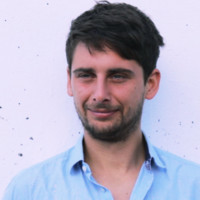
\includegraphics[width=0.6\columnwidth]{0.jpg} % REMOVE THIS LINE FOR NO PHOTO
\section{Contact}
+44 7379 433247
\href{mailto:joshuansjordan@gmail.com}{joshuansjordan\\@gmail.com}
\section{Languages}
C++, Python, C, C\#, Java, Lisp
\section{Tools}
OpenCV, Docker, Git, ZMQ, Darknet, Tensorflow, openVino, Numpy, matplotlib
\section{Platforms}
Linux, Windows, Nvidia Tx2, Raspberry Pi, Keil
\end{aside}

%----------------------------------------------------------------------------------------
%	Summary / intro
%----------------------------------------------------------------------------------------
\emph{I make solutions using software, creativity and machine learning. I'm passionate about working with great people to solve challenging problems that make a difference.}

\section{Experience}
%\begin{itemize}
- Excellent development ability in C++, Python and C\\
- Proven track record of idependently completing cutting-edge technology projects\\
- Responsible for system design of machine learning products\\
- Extensive experience with subversion, debugging tools and best practices\\
- Experience in designing real-time systems and optimization for embedded devices\\
- Interacted with clients and investors to scope computer vision products\\
- Excellent written and verbal communication skills\\
- Thrive within a creative team environment\\
- Constantly looking to learn and improve\\

%----------------------------------------------------------------------------------------
%	EMPLOYMENT SECTION
%----------------------------------------------------------------------------------------
\section{Employment}
\begin{entrylist}
%------------------------------------------------
\entry
{2017--2019}
{IMAGR - Mechatronics Engineer}
{www.imagr.co/}
{Key member in designing a world-class computer vision solution for retail. Saw our product go from early prototype to winning a contract with an international company and customer roll out. Real time detection and classification of >10,000 unique products.
\begin{itemize}
\item Rapid prototyping computer vision solutions
\item Designed an electro-mechanical autonomous data collection platform
\item Real-time deep learning classification and segmentation
\item "Big data" pipelines using zmq
\item Deep dive into camera systems
\item Helped set up the software team - hiring, testing and best practices
\item Liasion with investors, contractors and customers
\end{itemize}}

\entry
{2013--2017}
{Seequent (formaly AranzGeo) - Software Engineer}
{www.seequent.com/}
{Geological modelling startup producing best in class software in conjuction with a diverse team. Responible for critical features in the product.
\begin{itemize}
\item Implementation of complex mathematical code within a python/c codebase for windows
\item Fast, responsive and intuitive application with large datasets
\item Bug tracking, licensing and automated tests for desktop application
\end{itemize}}

\entry
{2012--2013}
{Trimble Navigation - Software Engineer}
{www.trimble.com/survey/}
{Developed innovative surveying products in a mature codebase to produce a wide range of geospatial data.
\begin{itemize}
\item Research and prototyping of real time HUD devices as an independent initiative
\item GPS and UX work in C and C++ for Windows CE devices
\item Developed an external API for third parties
\end{itemize}}

\entry
{2011-2012}
{HITLab NZ - Researcher}
{www.hitlabnz.org/}
{UX Research scholarship using a haptic device for molecular bonding problems.
\begin{itemize}
\item OpenGL and OpenCV development
\end{itemize}}
\end{entrylist}\\ 

%----------------------------------------------------------------------------------------
%	EDUCATION SECTION
%----------------------------------------------------------------------------------------
\section{Education}
\begin{entrylist}
\entry
{2007--2011}
{Bachelor of Engineering (Hons), Mechatronics}
{University of Canterbury, Christchurch}
{2:1 Distinction\\
Class representative - events organisation, liasion for peers}\\

\emph{Awards}\\
\entry
{2011}
{ENZCon published paper}
{Massey University, Palmerston North}
{Parallelism of an MCU on an FPGA}

\entry
{2007}
{McKee Trust Scholarship}
{University of Canterbury, Christchurch}
{Three year high achievement scholarship}
\end{entrylist}

\section{Volunteering}
\begin{entrylist}
\entry 
{2017-- }
{Event manger and artist}
{Hijinxx}
{Part of a community group running stages at various festivals in NZ. This involves Dj-ing, lighting setup and building artwork to engage and delight.} \\
\entry
{2015--}
{Start-up consultant}
{EasyLink}
{Technical consultant for feasibility of automated wheelchair system. Wrote all the software, including computer vision and controls, to get prototype ready for investor pitches.}
\end{entrylist}

\section{Interests}
\emph{Professional}\\ Artificial intelligence, embodied cognition, topology, computer vision, systems design, clean tech.\\
\\
\emph{Personal}\\ Surfing, DJ'ing, kite-surfing, football, sailing, guitar, skiing, acting.
\\ \\ \\ 
\emph{Written references available on request.}
\end{document}